\section*{Exercice 124 -- Torseurs dynamiques -- Orthèse}
\setcounter{exo}{0}
%Centrale Supelec PSI 2010


Soit le système suivant composé d'un bras et d'un avant-bras.

\begin{figure}[H]
\centering
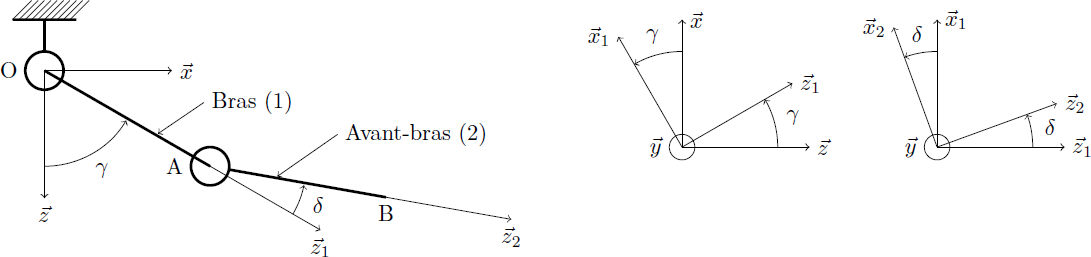
\includegraphics[width=\linewidth]{998_01}
\end{figure}

\begin{figure}[H]
\centering
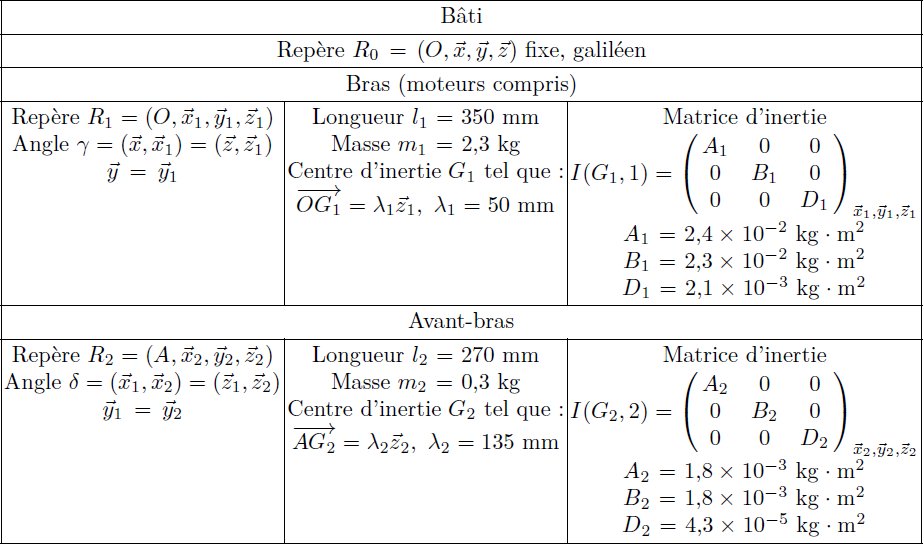
\includegraphics[width=\linewidth]{998_02}
\end{figure}

\subparagraph{}
\textit{Déterminer le torseur cinétique $\torseurcin{C}{\text{Bras}}{0}$ au point $O$ en utilisant deux méthodes différentes.}
\ifprof
\begin{corrige}
\end{corrige}
\else
\fi

\subparagraph{}
\textit{Déterminer le torseur dynamique $\torseurdyn{C}{\text{Bras}}{0}$ au point $O$ en utilisant deux méthodes différentes.}
\ifprof
\begin{corrige}
\end{corrige}
\else
\fi

\subparagraph{}
\textit{Déterminer le torseur cinétique $\torseurcin{C}{\text{Avant-Bras}}{0}$ au point $O$ en utilisant deux méthodes différentes.}
\ifprof
\begin{corrige}
\end{corrige}
\else
\fi

\subparagraph{}
\textit{Déterminer le torseur dynamique $\torseurdyn{\text{Avant-Bras}}{0}$ au point $O$ en utilisant deux méthodes différentes.}
\ifprof
\begin{corrige}
\end{corrige}
\else
\fi


\subparagraph{}
\textit{Déterminer le torseur dynamique $\torseurdyn{\text{Bras+Avant-Bras}}{0}$ au point $O$ en utilisant deux méthodes différentes.}
\ifprof
\begin{corrige}
\end{corrige}
\else
\fi

